% \titlepanel: the right of the title slide: a blue panel with a grain map
% coloured like an EBSD Euler map above the strength-elongation plane of the 25 measured alloys, their front
% dashed and a star beyond it; a red edge on its left. Inside a full-page tikzpicture[x=1mm,y=1mm] whose
% origin is the page's top-left corner, y downwards negative; the panel bleeds 1 mm past the edges.
\newcommand\titlepanel{%
  \fill[udsblue] (102,1) rectangle (161,-91);
  \node[anchor=north west,inner sep=0pt] (map) at (113.5,-11)
    {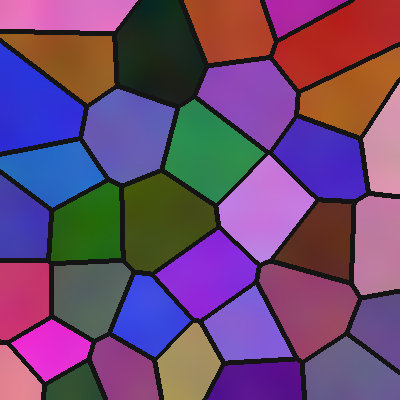
\includegraphics[width=36mm]{assets/drawn/grain-map}};
  \draw[white,line width=0.6pt] (map.south west) rectangle (map.north east);
  \draw[white,line width=0.9pt,-{Stealth[length=2mm,width=1.6mm]}] (131.5,-50.5) -- (131.5,-57);
  % the plane: 36 x 22 mm, yield strength 340-1000 MPa, elongation 30-86 %
  \begin{scope}[shift={(113.5,-83)}]
    \draw[white,line width=0.7pt] (0,22) -- (0,0) -- (36,0);
    \begin{scope}[x=0.054545mm,y=0.392857mm,shift={(-340,-30)}]
      \drawfront[white!75!udsblue,line width=0.6pt,dash pattern=on 1.4pt off 1pt]
      \foreach \s/\e/\i in \alloydata
        \node[circle,fill=white!85!udsblue,inner sep=0pt,minimum size=1.1mm] at (\s,\e) {};
      \node[circle,fill=white,inner sep=0pt,minimum size=4.6mm] (star) at (790,64) {};
      \node[text=udsred,font=\footnotesize] at (star) {\faStar};
    \end{scope}
  \end{scope}
  \fill[udsred] (102,1) rectangle (103.6,-91);}

% \doiline: https://doi.org/ and the paper's DOI, as a link in the slides; in the speaker notes, whose
% thumbnails scale the slide but not its links, the same text without a link
\newcommand\audiencemode{hide notes}
\ifx\notesmode\audiencemode
  \newcommand\doiline{\href{https://doi.org/\paperdoi}{https://doi.org/\paperdoi}}
\else
  \newcommand\doiline{\textcolor{udsblue}{https://doi.org/\paperdoi}}
\fi

% ------------------------------------------------------------------ title
\begin{frame}[plain,noframenumbering]
% Drawn inside the frame rather than over the page, so the speaker notes' thumbnail shows it too.
% The picture's origin is the page's top-left corner: a plain frame's body starts 8 mm in and
% 2 mm down.
\vbox to 0pt{\vskip-2mm\hbox to 0pt{\hskip-8mm\begin{tikzpicture}[x=1mm,y=1mm]
  \useasboundingbox (0,0) rectangle (160,-90);
  \titlepanel
  \node[anchor=north west,inner sep=0pt] at (8,-8) {\includegraphics[width=30mm]{\udslogo}};
  % the text block grows upwards from the presenter's name, whose baseline stays 66.5 mm from the top,
  % at the same distance from the d3M block as in the Coding Agents talk; the citation and the DOI under
  % it form one block, and the red rule sits halfway between that block and the name
  \node[anchor=south west,inner sep=0pt,text width=90mm,align=left,
    execute at begin node={\hyphenpenalty=10000\exhyphenpenalty=10000}] at (8,-66.63) {%
    {\fontsize{16.5}{18}\selectfont\bfseries\color{udsblue}\inserttitle\par}\vskip2mm
    {\fontsize{12}{14.5}\selectfont\color{udsdark}\insertsubtitle\par}\vskip0.6mm
    {\fontsize{9}{11}\selectfont\doiline\par}\vskip1.25mm
    \textcolor{udsred}{\rule{14mm}{0.8pt}}\par\vskip3mm
    {\fontsize{11}{13}\selectfont\color{udsdark}\insertauthor\par}};
  \node[anchor=south west,inner sep=0pt] (d3m) at (8,-83) {
\includegraphics[width=10mm]{assets/d3m.png}};
  \node[anchor=west,inner sep=0pt,text width=74mm,align=left,font=\fontsize{7}{8.8}\selectfont,
    execute at begin node={\hyphenpenalty=10000}] at ([xshift=3mm]d3m.east) {%
    {\color{udsblue}\insertinstitute\par}
    {\color{udsgrey}\insertdate\par}};
\end{tikzpicture}\hss}\vss}
% a frame with no tall content drops out of the notes' thumbnail; this invisible strut keeps it
\par\rule{0pt}{80mm}
\note{\textbf{0:00--0:20}\par
    A paper from Nature Communications, published at the end of September 2026.\par
    The authors train generative models on electron backscatter diffraction (EBSD) maps of 25 variants of
      one alloy, and search them for microstructures that are both stronger and more ductile.\par
    I follow the paper's own story.}
\end{frame}

% ---------------------------------------------------------------- outline
\begin{frame}{Outline}
  % each section's title as on its divider, and the divider's question
  \small\renewcommand\arraystretch{1.4}\setlength\tabcolsep{4pt}
  \begin{tabularx}{\textwidth}{@{}>{\leavevmode\color{udsblue}\bfseries}p{4mm}>{\bfseries}p{42mm}X@{}}
    \toprule
    1 & The design problem   & Why ask a generative model for new microstructures?\\
    2 & Groundwork           & Which methods does the paper build on?\\
    3 & The method           & How are microstructures generated and steered toward properties?\\
    4 & The results          & What do the authors show?\\
    \bottomrule
  \end{tabularx}
  \note{\textbf{0:20--0:50}\par
    Four sections, each answering one question.\par
    Section 2 introduces the machine-learning methods the paper combines, with their origins, for anyone
      who has not followed that literature.\par
    Sections 3 and 4 present the paper as the authors tell it.}
\end{frame}
